\chapter{Methodology}
\label{sec:methodology}

\begin{German}
    Gemäss Creswell \cite{creswellHttpsWwwucgacmeSkladiste} werden vier Paradigmen vorgeschlagen, um neues wissenschaftliches Wissen zu generien: Postpositivismus, Konstruktivismus, Transformatives Paradigma sowie Pragmatismus. Pragmatismus ist ein erkenntnistheoretisches Paradigma. Wahrheit wird als das bewertet, was in der Praxis funktioniert. Forschung wird damit als zielgerichtetes Mittel zur Lösung konkreter Probleme verstanden.
    
    Ein Forschungsansatz innerhalb des Pragmatismus ist Design Science Research (DSR) \cite{desordiDesignScienceResearch2021}. Er stammt aus den Ingenieur- und Informationswissenschaften und wird im Rahmen dieser Arbeit angewendet. Es werden innovative Artefakte entwickelt um reale Probleme zu lösen. Gleichzeitig soll die Forschung wissenschaftlich fundiert sein und neues Wissen generieren, das über den Einzelfall hinaus generalisierbar ist. DSR verbindet somit praktische Nützlichkeit mit theoretischem Erkenntnisgewinn.
            
    Zur Anwendung von Design Science Research als Methodik stehen verschiedene methodologische Ansätze zur Verfügung. Das am weitest verbreiteste \cite{desordiDesignScienceResearch2021} ist die Design Science Research Methodology (DSRM) von Peffers et al \cite{peffersPDFDesignScience2024}. "Without a framework that is shared by authors, reviewers, and editors, DS research runs the danger of being mistaken for poor-quality empirical research or for practice case study" \cite{peffersPDFDesignScience2024}. Um dies zu vermeiden werden sechs Schritte vorgeschlagen (vgl. \ref{fig:DSR}). Die einzelnen Schritte werden in den folgenden Kapiteln jeweils aufgegriffen und umgesetzt (vgl. \ref{tab:DSRM_steps}):
\end{German}

\begin{English}
    According to Creswell \cite{creswellHttpsWwwucgacmeSkladiste}, four paradigms are proposed to generate new scientific knowledge: postpositivism, constructivism, transformative paradigm, and pragmatism. Pragmatism is an epistemological paradigm. Truth is evaluated as what works in practice. Research is thus understood as a goal-oriented means to solve concrete problems. 
    
    A research approach within pragmatism is Design Science Research (DSR) \cite{desordiDesignScienceResearch2021}. It originates from engineering and information sciences and is applied in this work. Innovative artifacts are developed to solve real problems. At the same time, the research should be scientifically founded and generate new knowledge that is generalizable beyond the individual case. DSR thus combines practical utility with theoretical knowledge gain.
            
    To apply Design Science Research as a methodology, various methodological approaches are available. The most widespread \cite{desordiDesignScienceResearch2021} is the Design Science Research Methodology (DSRM) by Peffers et al \cite{peffersPDFDesignScience2024}. "Without a framework that is shared by authors, reviewers, and editors, DS research runs the danger of being mistaken for poor-quality empirical research or for practice case study" \cite{peffersPDFDesignScience2024}. To avoid this, six steps are proposed (see fig. \ref{fig:DSR}). The individual steps are taken up and implemented in the following chapters (see tab. \ref{tab:DSRM_steps}).
\end{English}

\begin{table}[htbp]
    \centering
    \begin{tabular}{ll}
    \toprule
    \textbf{DSRM Step} & \textbf{Thesis Chapter} \\
    \midrule
    1. Problem Identification and Motivation & \ref{sec:background_motivation}, \ref{sec:problem_identification} \\
    2. Definition of the Objectives for a Solution & \ref{sec:research_objectives}, \ref{sec:objectives} \\
    3. Design and Development & \ref{sec:design_development} \\
    4. Demonstration & \ref{sec:case_study} \\
    5. Evaluation & \ref{sec:results}, \ref{sec:discussion} \\
    6. Communication & \ref{sec:conclusion} \\
    \bottomrule
    \end{tabular}
    \caption{Mapping of DSRM steps to thesis chapters}
    \label{tab:DSRM_steps}
\end{table}

\begin{German}
    Die DSRM wurde gewählt, weil sie sich besonders gut für die systeamtische Entwicklung und Evalutaion technischer Artefakte eignet. Sie ermöglicht ein strukturiertes Vorgehen zur Erstellung eines automatisierten Scan-to-BIM-Framework, der ein reales, praxisrelevantes Problem adressiert. Gleichzeitig gewährleistet sie eine wissenschaftlich fundierte Herleitung und Bewertung der entwickelten Lösung.
\end{German}

\begin{English}
    The DSRM was chosen because it is particularly well suited for the systematic development and evaluation of technical artifacts. It enables a structured approach to create an automated Scan-to-BIM framework that addresses a real, practice-relevant problem. At the same time, it ensures a scientifically founded derivation and evaluation of the developed solution.
\end{English}
    
\begin{figure}[h]
    \centering
    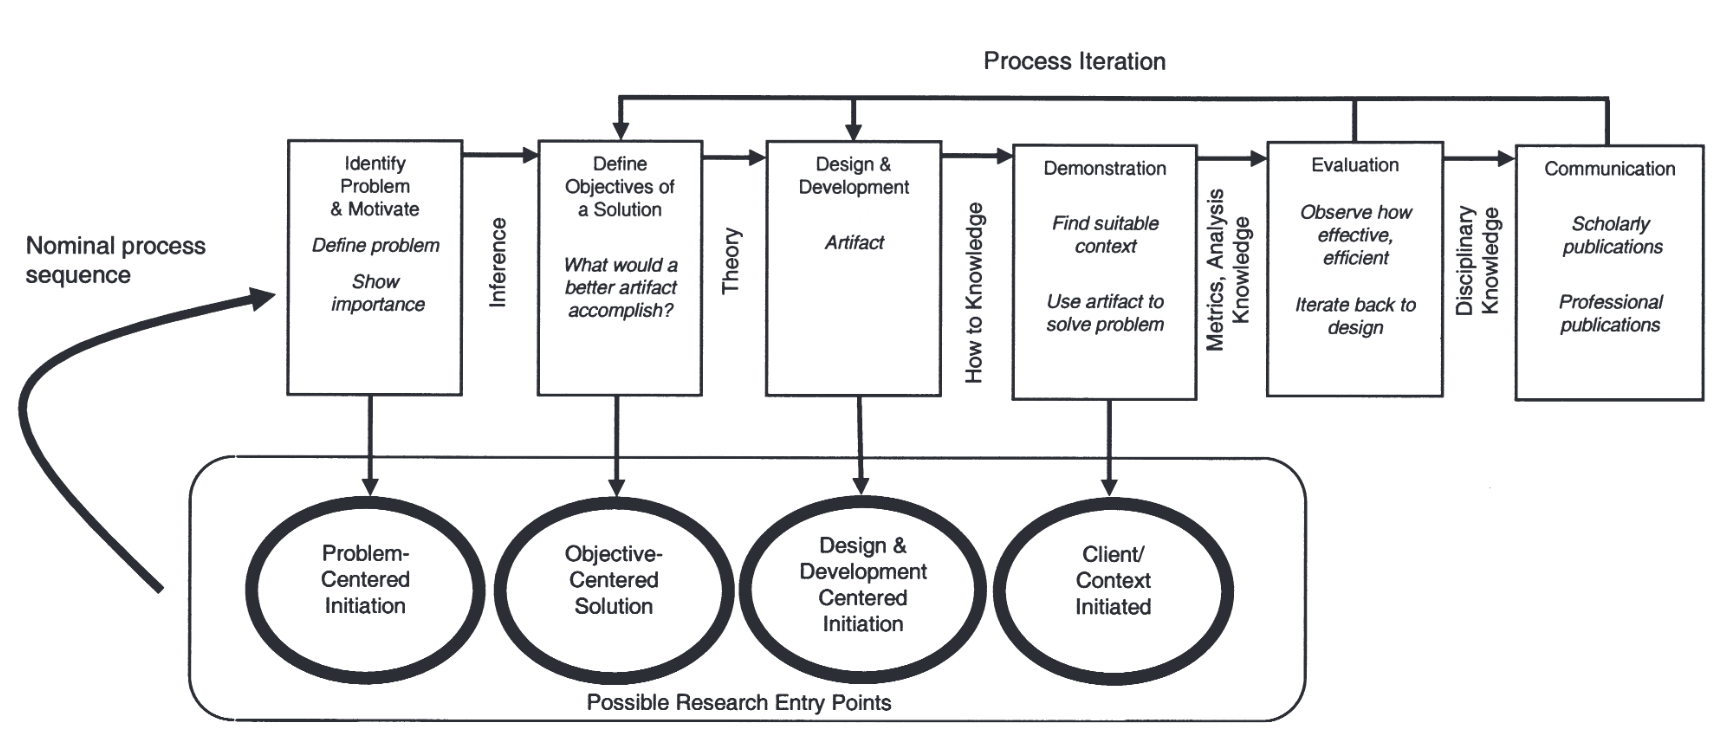
\includegraphics[width=1\textwidth]{images/DSR.png}
    \caption{Design Science Research Methodology (DSRM) \cite{peffersPDFDesignScience2024}}
    \label{fig:DSR}
\end{figure}

\section{Problem Identification and Motivation}
\label{sec:problem_identification}
\begin{German}
    Auf das generelle Problem der Branche wurde bereits in der Einführung (vgl. \ref{sec:introduction}) eingegangen. Nun soll die Brücke zur konkreten Problemstellung geschlagen werden, die im Rahmen dieser Arbeit adressiert wird. Die Arbeit entstand in Zusammenarbeit mit Axians Schweiz, einem Unternehmensverbund mit rund 940 Mitarbeitenden \cite{AxiansSchweiz}. Axians ist die ICT-Marke von VINCI Energies, einem Geschäftsbereich des französischen Konzerns VINCI. Mit rund 285.000 Mitarbeitenden \cite{VINCI2025} zählt VINCI zu einem der weltweit grössten Unternehmen im Bereich Bau, Infrastruktur und Konzessionen.
\end{German}
    
\begin{English}
    The general problem of the industry has already been addressed in the introduction (see \ref{sec:introduction}). Now, the bridge to the concrete problem that is addressed in this work should be built. The work was created in collaboration with Axians Switzerland, a corporate group with around 940 employees \cite{AxiansSchweiz}. Axians is the ICT brand of VINCI Energies, a business unit of the French group VINCI. With around 285,000 employees \cite{VINCI2025}, VINCI is one of the largest companies in the field of construction, infrastructure, and concessions worldwide.
\end{English}
  

\section{Definition of the Objectives for a Solution}
\label{sec:objectives}

\section{Design and Development}
\label{sec:design_development}
